\documentclass[11pt,a4paper]{article}
\usepackage[T1]{fontenc}
\usepackage[utf8]{inputenc}
\usepackage{lmodern}
\usepackage[margin=1in]{geometry}
\usepackage{microtype}
\usepackage{hyperref}
\usepackage{graphicx}
\usepackage[space]{grffile}
\usepackage{xstring}
\usepackage{siunitx}
\usepackage{caption}
\captionsetup{font=small}
\usepackage{setspace}
\usepackage{titlesec}
\usepackage{xcolor}
\usepackage{hyperref}
\usepackage{enumitem}
\usepackage{graphicx}
\usepackage{booktabs}
\usepackage{listings}
\usepackage{caption}
\usepackage{minted}
\usepackage{siunitx}
\usepackage{graphicx}
\usepackage{tikz}
\usetikzlibrary{arrows.meta, positioning}
\usepackage[space]{grffile}

\newcommand{\locustwide}[1]{\includegraphics[width=.55\linewidth]{#1}}
\newcommand{\locustnarrow}[1]{\includegraphics[width=.45\linewidth]{#1}}
\newcommand{\lambdawide}[1]{\includegraphics[width=.92\linewidth]{#1}}
\newcommand{\lambdahalf}[1]{\includegraphics[width=.70\linewidth]{#1}}


\newcommand{\scenariofig}[4][\linewidth]{%
  \begin{figure}[htbp]
    \centering
    \includegraphics[width=#1]{#2}
    \caption{#3}
    \label{#4}
  \end{figure}%
}


\hypersetup{
  colorlinks=true,
  linkcolor=black,
  urlcolor=blue,
  citecolor=black,
  pdfauthor={<Your Name>},
  pdftitle={Serverless Named Entity Recognition on AWS Lambda},
  pdfsubject={Cloud Computing Project Report},
  pdfkeywords={AWS Lambda, API Gateway, SAM, spaCy, NER, Serverless, CloudWatch, Locust}
}

\lstdefinestyle{code}{
  basicstyle=\ttfamily\small,
  keywordstyle=\bfseries\color{black},
  commentstyle=\itshape\color{gray!70!black},
  stringstyle=\color{teal!60!black},
  showstringspaces=false,
  frame=single,
  framerule=0.3pt,
  rulecolor=\color{black!20},
  breaklines=true,
  columns=fullflexible
}
\lstset{style=code}

\makeatletter
\let\orig@includegraphics\includegraphics
\renewcommand{\includegraphics}[2][]{%
  \begingroup
    \def\imgfile{#2}%
    % Locust - Charts
    \IfSubStr{\imgfile}{Charts}{%
      \orig@includegraphics[width=.55\linewidth]{#2}%
    }{%
      % Locust - Stats
      \IfSubStr{\imgfile}{Stats}{%
        \orig@includegraphics[width=.45\linewidth]{#2}%
      }{%
        % Lambda metrics
        \IfSubStr{\imgfile}{Duration}{%
          \orig@includegraphics[width=.70\linewidth]{#2}%
        }{%
          \IfSubStr{\imgfile}{Invocation}{%
            \orig@includegraphics[width=.70\linewidth]{#2}%
          }{%
            \IfSubStr{\imgfile}{Invocations}{%
              \orig@includegraphics[width=.70\linewidth]{#2}%
            }{%
              \IfSubStr{\imgfile}{Concurrent}{%
                \orig@includegraphics[width=.70\linewidth]{#2}%
              }{%
                \IfSubStr{\imgfile}{ConcEx}{%
                  \orig@includegraphics[width=.70\linewidth]{#2}%
                }{%
                  % default
                  \orig@includegraphics[width=\linewidth]{#2}%
                }%
              }%
            }%
          }%
        }%
      }%
    }%
  \endgroup
}
\makeatother

\title{\vspace{-1.5em}\Large\bfseries Serverless Named Entity Recognition on AWS Lambda}
\author{Riccardo Pitzanti - 1947877 \quad \quad \quad \quad Federico Iannini - 1931748\\
  \normalsize pitzanti.1947877@studenti.uniroma1.it \quad iannini.1931748@studenti.uniroma1.it\\[0.25em]
  \normalsize Sapienza Università di Roma}
\date{\normalsize \today}

\begin{document}
\maketitle
\vspace{-1.5em}

\section{Introduction}
This work explores the application of a production-ready NLP pipeline for Named Entity Recognition (NER) on AWS Lambda. By leveraging AWS Lambda and Amazon API Gateway, we architect a microservice that is inherently scalable. The implementation utilizes the spaCy library, whilst the entire application stack—including compute, API management, and security—is defined and deployed using the AWS Serverless Application Model (SAM).

The primary objective of this study is to design and evaluate the performance characteristics of this service under varied load conditions. We employ Locust, an open-source load-testing tool, to simulate traffic patterns. The findings confirm the viability of serverless architectures for deploying microservices.

\section{Background}

\subsection{Named Entity Recognition (NER) and spaCy}
NER is a NLP task focused on identifying and categorizing information elements, known as entities, within unstructured text. These entities are typically classified into predefined categories such as persons (\textsf{PERSON}), organizations (\textsf{ORG}), and geopolitical entities (\textsf{GPE}). The spaCy library in Python provides a framework for implementing NLP pipelines, offering statistical models for tasks like NER.
The choice of NER as the target workload, rather than other AI models is motivated by its balance of practical relevance and clear performance indicators. NER is a core component of many real-world applications where extracting structured information from unstructured text is essential. Application fields include news and document analytics, compliance monitoring, biomedical literature mining, customer support automation, and conversational agents.


\subsection{AWS SAM \& Containerized Build with Docker}
The AWS Serverless Application Model (SAM) is an open-source framework that extends AWS CloudFormation to provide a simplified syntax for defining serverless resources. It is a form of Infrastructure as Code (IaC) specifically designed to express the functions, APIs, permissions, and events that compose a serverless application. A containerized build process involves using an isolated environment to compile application dependencies and package the code. By employing Docker, in our case, SAM ensures that the build process is executed within a containerized environment that replicates the AWS Lambda runtime. This guarantees consistency between the development build and the deployment target, thereby mitigating compatibility issues.

\subsection{AWS Lambda and HTTP API}
AWS Lambda is a serverless, event-driven compute service that allows for the execution of code in response to triggers without requiring the management of underlying servers. It automatically scales with incoming request volume and utilizes a fine-grained cost model based on actual compute consumption. The Amazon API Gateway is a fully managed service that simplifies the deployment of APIs at any scale.

\subsection{Observability with CloudWatch}
Observability is a system property that describes how well internal states can be understood from external outputs, primarily through the collection and analysis of logs, metrics, and traces. Amazon CloudWatch is a monitoring and observability service that provides a unified view of AWS resources. It automatically collects performance metrics from services like AWS Lambda.

\subsection{Load Testing with Locust}
Locust is an open-source load testing tool that allows developers to define user behavior with Python code and simulate various concurrent users to assess a system's performance under stress. Its distributed and scalable nature makes it suitable for testing the limits of web services and APIs. It provides a real-time web-based user interface to visualize performance indicators such as requests per second, response times, and the number of failing requests as the test is running.

\section{System Design and Implementation}
\begin{figure}[h]
\centering
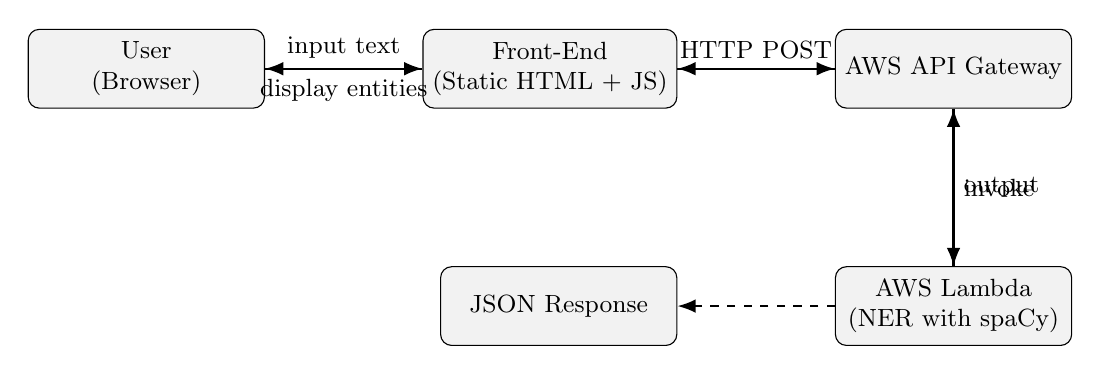
\begin{tikzpicture}[
    node distance=2cm,
    every node/.style={align=center, font=\small},
    box/.style={rectangle, draw, rounded corners, minimum width=3cm, minimum height=1cm, fill=gray!10},
    arrow/.style={-Latex, thick}
]

% Nodes
\node[box] (user) {User \\ (Browser)};
\node[box, right=of user] (frontend) {Front-End \\ (Static HTML + JS)};
\node[box, right=of frontend] (apigw) {AWS API Gateway};
\node[box, below=of apigw] (lambda) {AWS Lambda \\ (NER with spaCy)};
\node[box, left=of lambda] (response) {JSON Response};

% Arrows
\draw[arrow] (user) -- (frontend) node[midway, above] {input text};
\draw[arrow] (frontend) -- (apigw) node[midway, above] {HTTP POST};
\draw[arrow] (apigw) -- (lambda) node[midway, right] {invoke};
\draw[arrow] (lambda) -- (apigw) node[midway, right] {output};
\draw[arrow] (apigw) -- (frontend);
\draw[arrow] (frontend) -- (user) node[midway, below] {display entities};

% Optional response box
\draw[arrow, dashed] (lambda.west) -- (response.east);

\end{tikzpicture}
\caption{System architecture of the NER Lambda application.}
\end{figure}


\noindent\textbf{API contract.}
\begin{minted}[
    frame=single,
    linenos
  ]{json}
POST /ner
Content-Type: application/json
{"text": "Alan Turing was born on June 23, 1912, in London, England."}

200 OK
{"entities": [
    {'text': 'Alan Turing', 'label': 'PERSON', 'start': 0, 'end': 11},
    {'text': 'June 23, 1912', 'label': 'DATE', 'start': 24, 'end': 37},
    {'text': 'London', 'label': 'GPE', 'start': 41, 'end': 47},
    {'text': 'England', 'label': 'GPE', 'start': 49, 'end': 56}]
}
\end{minted}
%caption={Request and response schemas (illustrative).}


\section{Methodology and Implementation}

\subsection{Inference Module (\texttt{src/ner.py})}
This module is responsible for the NER task: it utilizes the spaCy library, a framework for NLP in Python. The pre-trained model (\texttt{en\_core\_web\_sm}) is loaded into a global constant at module import time. The primary function, \texttt{extract\_entities(text: str)}, processes an input string through the spaCy pipeline. It returns a list of dictionaries, each containing the extracted entity's surface form (\texttt{text}), its ontological class (\texttt{label}), and the character-level indices (\texttt{start}, \texttt{end}) denoting its span within the original text.

\subsection{Lambda Handler Function (\texttt{src/handler.py})}
This module implements the AWS Lambda function handler, which serves as the entry point for requests proxied by Amazon API Gateway. Its primary role is to manage the HTTP request-response cycle. The handler first invokes a helper function, \texttt{\_parse\_body}, to normalize the incoming event structure. This function abstracts away the differences between the event payload delivered by API Gateway (where the HTTP request body is passed as a JSON-encoded string) and the event object used during local testing (which may be a Python dictionary). The handler then performs input validation, checking for the presence and type of the required \texttt{'text'} field. Invalid requests result in a \texttt{400 Bad Request} response. Validated text is passed to the inference core, and the resulting entities are serialized into a JSON object returned within a \texttt{200 OK} response.

\subsection{Build Process}
The build is executed using the AWS SAM CLI command \texttt{sam build --use-container}. This process constructs the deployment package inside a Docker container that emulates the Amazon Linux environment of AWS Lambda.

\subsection{Infrastructure Provisioning (SAM Template)}
The cloud infrastructure is defined declaratively using the AWS Serverless Application Model. The template, \texttt{template.yaml}, specifies a minimal and functional stack:
\begin{itemize}
    \item A single AWS Lambda function resource with its runtime (\texttt{python3.9}), allocated memory (512 MB), and timeout (15 seconds) defined in the \texttt{Globals} section.
    \item An Amazon API Gateway HTTP API resource, which provisions a managed HTTPS endpoint. This API is configured with a single route (\texttt{POST /ner}) that integrates directly with the Lambda function.
    \item A pre-existing IAM role (\texttt{LabRole}) is referenced for execution permissions, a constraint of the AWS Academy Learner Lab environment. In a standard AWS account, SAM would typically generate a minimal role with necessary permissions automatically.
\end{itemize}

\subsection{Front-End}
The front-end component of the application is deliberately designed as a minimal web interface to facilitate testing and demonstration of the deployed NER service. It is implemented as a static \texttt{HTML} page with basic \texttt{JavaScript} logic. 
\section{Performance Evaluation and Testing}\label{sec:testing}

\subsection{Goals and approach}
The objective is to evaluate the responsiveness, scalability, and stability of the NER microservice deployed on AWS Lambda. Each experiment uses a structured workload with \emph{Warm-up (WU)}, \emph{Ramp-up (RU)}, \emph{Steady (S)}, and \emph{Ramp-down (RD)} phases. We collect both \emph{user-oriented} (client) and \emph{system-oriented} (provider) metrics and align the CloudWatch time windows with the Locust test window (WU excluded).

\subsection{Common settings across all scenarios}
The experiments share a set of common settings. First, a Warm-up (WU) phase of \SI{60}{s} at 2 users (spawn rate 2/s) is executed in order to trigger cold starts. Immediately after the warm-up phase the client statistics are reset so that the run-up, steady, and run-down periods are isolated in the reported numbers. The payload mix consists of short and long English sentences containing named entities such as persons, organizations, locations, and dates; requests are performed via POST /ner with a small JSON body. Each scenario is executed in both a \emph{Light} and a \emph{Heavy} profile: the Light profile uses lower request rates per second (RPS) with more realistic user pacing, while the Heavy profile uses higher RPS and near-zero client think time to approach the Lambda concurrency ceiling.

\subsection{Workload scenarios}
We use three canonical workload shapes as a methodological basis to stress different operational aspects of the system under test, as depicted in Table 1. Durations reported below always refer to the \emph{main window} (after the warm-up and statistics reset). ``Users'' denote active virtual users, while the effective request rate (RPS) emerges from the interplay of user count, client think time, and function latency. The selection of these three shapes is motivated by the need to emulate diverse yet representative access patterns. The \emph{Bursty} scenario models sustained but intermittent interaction, suitable for capturing cold start recovery and concurrency stabilization. The \emph{Ramp--Steady--Ramp-down} scenario represents a gradual increase in load, followed by a sustained plateau and subsequent decrease, which allows evaluation of scaling dynamics. The \emph{Spike} scenario emulates sudden surges of demand, providing insights into system responsiveness under rapid load fluctuations.

\begin{table}[h]
\centering
\renewcommand{\arraystretch}{1.3}
\begin{tabular}{|p{2cm}|p{2cm}|p{10cm}|}
\hline
\textbf{Scenario} & \textbf{Profile} & \textbf{Description} \\
\hline

A — Bursty &
Light A &
Constant 5 users for \SI{300}{s}; long think time (5–10\,s) to emulate intermittent clicks $\Rightarrow$ low, flat RPS plateau. \\
\cline{2-3}
& Heavy A &
Constant 10 users for $\approx$\SI{360}{s}; near-zero think time (0–0.1\,s) to drive high RPS until bounded by Lambda concurrency. \\
\hline

B — Ramp $\rightarrow$ Steady $\rightarrow$ Ramp-down &
Light B &
RU in \SI{60}{s} steps through 1$\rightarrow$3$\rightarrow$5$\rightarrow$6$\rightarrow$7$\rightarrow$8 users, then S at 8 users for \SI{240}{s}, then RD 4 users (\SI{60}{s}) and 1 user (\SI{60}{s}). Think time short (0.2–1.0\,s). \\
\cline{2-3}
& Heavy B &
Faster RU to 10 users, S at 10 users for $\approx$\SI{240}{s}, then RD; near-zero think time (0–0.1\,s) for high RPS. \\
\cline{2-3}
& Vertical scaling &
Heavy~B executed twice with identical shape, once at \SI{512}{MB} and once at \SI{1024}{MB}, to quantify the impact of memory on latency (p95/p99) and steady-state throughput. \\
\hline

C — Spike &
Light C &
Pre-spike \SI{30}{s} at 1 user, spike to 8 users for \SI{240}{s}, then \SI{60}{s} at 2 users; short think time (0.2–1.0\,s). \\
\cline{2-3}
& Heavy C &
Pre-spike \SI{30}{s} at 2 users, spike to 10 users for \SI{240}{s}, then \SI{60}{s} at 2 users; near-zero think time (0–0.1\,s). \\
\hline

\end{tabular}
\caption{Definition of workload scenarios (Light and Heavy profiles).}
\end{table}

\subsection{Extra: Stress test scenario}
The decision to conduct a stress test, even with the known constraint of the AWS Learner Lab's resource limits, was a calculated one aimed at challenging the boundaries of the serverless architecture. While the used account was eventually suspended for exceeding its concurrency quota (10 concurrent executions), the outcome itself was a valuable data point. Crucially, the client-side metrics collected by Locust prior to the suspension were preserved. However, CloudWatch metrics were not available after the run, due to the account's suspension. The stress test scenario was therefore executed with a shortened 3-minute window to probe headroom while staying within budget.
\paragraph{Test composition and outcome (\emph{Very Heavy A} “\texttt{hhA}”).}
To probe headroom beyond the Heavy envelope, we executed a more aggressive variant of scenario~A using the settings captured in \texttt{hhA - Charts.png} and \texttt{hhA - Stats.png}. Warm-up was shortened and the active user pool enlarged to drive a higher arrival rate while keeping per-user think time minimal.

\begin{table}[h]
\centering
\small
\caption{Test composition for the \emph{Very Heavy A} (\texttt{hhA}) stress run.}
\label{tab:hhA-plan}
\begin{tabular}{llccc}
\toprule
Stage & Duration & Active users & Spawn behavior & Per-user think time \\
\midrule
Warm-up (WU) & 30\,s  & 2 & 2\,users/s (WU only) & near-zero \\
Main window  & 180\,s & 40 (steady plateau) & rapid climb after WU & $\approx$0--0.1\,s \\
\bottomrule
\end{tabular}
\end{table}

\noindent\textbf{Observed outcome (Locust).}
From the \texttt{hhA} charts/stats:
(i) sustained throughput at $\sim$60--70\,req/s across the steady window with \emph{zero failures};
(ii) latency stabilizes after the brief WU spike with p50 $\approx$ 0.64\,s and p95 $\approx$ 0.73\,s;
(iii) a single max-latency outlier around $\sim$6.9\,s occurs at the transition and does not persist in steady state.
Given the 180\,s main window, this corresponds to roughly $1.1\times 10^4$--$1.3\times 10^4$ successful requests in steady state.

\begin{table}[h]
\centering
\small
\caption{Summary metrics for \texttt{hhA} (from \texttt{hhA - Stats.png}/\texttt{hhA - Charts.png}).}
\label{tab:hhA-metrics}
\begin{tabular}{lcccccc}
\toprule
Window & Plateau RPS & Failures & p50 (s) & p95 (s) & Max (s) & Notes \\
\midrule
180\,s (steady) & $\sim$60--70 & 0 & 0.64 & 0.73 & $\sim$6.9 & single outlier at transition \\
\bottomrule
\end{tabular}
\end{table}

\noindent\textbf{Interpretation.}
Despite the learner-lab concurrency ceiling and the shortened window, the client-side evidence indicates the system absorbed the higher arrival rate without degradation in the steady segment: throughput rose with load, medians remained low, and tails stayed bounded aside from the expected warm-up/transition blip. As noted above, CloudWatch provider-side series are unavailable post-run due to account suspension, so conclusions for \texttt{hhA} rest on the preserved Locust artifacts.

\section{Results and discussion}
% OK part
The primary objective of this evaluation is to assess whether the system under study maintains its service quality under stress conditions. 
Before examining the results, it is useful to clarify how the reported charts and metrics should be read and interpreted. The Locust charts primarily display the evolution of requests per second (RPS) together with latency percentiles (p50, p95, p99). The RPS curve reflects the effective throughput generated by the virtual users, while the percentile lines capture the distribution of response times. When both curves settle into a stable plateau, this indicates that the system has reached a steady operating state.
Complementing these charts, the Locust request statistics provide aggregated values of latency percentiles, request counts, and possible failures, thereby allowing the tails of the latency distribution and the presence or absence of execution errors to be assessed at a glance. On the provider side, the AWS Lambda metrics add further explanatory depth. The \emph{Invocations} series tracks the cumulative number of requests served, where a linear slope corresponds to constant throughput. The \emph{ConcurrentExecutions} metric shows the number of function instances active at a given moment, thus making concurrency ceilings and the elasticity of scaling behavior visible. The \emph{Duration} series measures execution time per invocation, with narrow and stable bands signifying predictable performance and wider fluctuations revealing potential variability. 

% Not OK part (replaced)
Our reading of the experiments is two-sided and evidence-led. First, we \emph{cross-check throughput} by comparing Locust RPS with the slope of CloudWatch \emph{Invocations}; the two match in shape and level during steady windows, confirming that client-side and provider-side views are consistent. Second, we \emph{validate elasticity} by verifying that \emph{ConcurrentExecutions} rises and falls with the arrival rate (bursts, ramps, and spikes) and returns to baseline after load drops, indicating healthy scale-out/scale-in. Third, we \emph{bound latency} using Locust percentiles: p50 captures the typical user experience, while p95/p99 quantify tail behavior; brief transitions (ramp steps and spikes) are assessed separately from steady windows. Finally, we \emph{scan for stress signals}—failures in Locust, and visual cues of throttling or saturation in CloudWatch (e.g., a flat concurrency ceiling or diverging RPS vs.\ invocations). This procedure removes ambiguity between client pacing and backend capacity and ties each conclusion to a specific metric.

% Not OK part (replaced)
Across all shapes, the service sustains steady throughput with low median latency and bounded tails, without recorded request failures. In the \textbf{Heavy} profile, Locust reports \(\text{RPS} \in [23.06, 30.72]\) with scenario medians p50 \(=170\text{--}180\,\mathrm{ms}\) and p95 \(=390\text{--}580\,\mathrm{ms}\) (p99 \(=840\text{--}1100\,\mathrm{ms}\)); the highest observed steady-state throughput is \(\mathbf{30.72}\,\mathrm{req/s}\) in Heavy~A (bursty). In the \textbf{Light} profile, throughput spans \(\text{RPS} \in [17.90, 22.01]\) with p50 \(=170\text{--}330\,\mathrm{ms}\), p95 \(=370\text{--}480\,\mathrm{ms}\), and p99 \(\le 500\,\mathrm{ms}\). Max latencies of \(4\text{--}5\,\mathrm{s}\) appear as rare outliers that coincide with abrupt fan-out (spikes/step-ups), a pattern consistent with cold starts rather than sustained saturation. CloudWatch corroborates these patterns: \emph{ConcurrentExecutions} traces mirror the input shapes (bursts, ramps, spikes), \emph{Invocations} grow linearly during steady windows (constant effective throughput), and \emph{Duration} bands remain tight once warm. No evidence of a hard concurrency ceiling or plateaued throughput is visible in any scenario, which supports the conclusion that the application scales elastically within the tested load envelope.

% OK part
The RU/S/RD structure in B and the transient spike in C produce brief, expected percentile spikes at transitions; the system stabilizes quickly in the steady segment with no persistent oscillations.
No sustained errors or throttles were observed in Locust or CloudWatch during the steady windows. Availability therefore remained effectively \(> 99.9\%\) for the windows considered; brief spikes during transitions are attributed to cold-starts or step changes and do not persist.

\section{Conclusion}\label{sec:conclusion}

We evaluated a serverless NER API on AWS Lambda behind API Gateway using three canonical workload shapes (A: bursty, B: ramp–steady–ramp, C: spike), each in \emph{Light} and \emph{Heavy} variants, plus targeted vertical scaling experiments and an heavier stress test. An additional stress test scenario was executed with a shortened 3-minute plan.
Within the tested limits, the architecture \emph{scales accordingly and efficiently}: throughput increases with client concurrency, latency remains controlled and predictable after warm-up, and vertical scaling via memory provides a clear performance uplift when needed. The system shows no anomalous behavior under bursty, ramped, or spiky demand, and maintains zero-failure operation at the highest tested loads (stress test).
Future work could focus on refining both the scalability experiments and the methodology for measurement. On the experimental side, one direction could be to extend the range of load profiles beyond the canonical shapes used in this work or to explore other workload patterns. On the methodological side, we could investigate the impact of different client-side configurations on the observed behavior, such as varying think times or concurrency levels.

\scenariofig{figures/hA - Charts.png}{Heavy A — Locust RPS and latency percentiles.}{fig:ha-charts}
\scenariofig{figures/hA - Stats.png}{Heavy A — Locust request statistics.}{fig:ha-stats}
\scenariofig{figures/hA - Invocations.png}{Heavy A — Lambda Invocations (provider-side throughput).}{fig:ha-invocations}
\scenariofig{figures/hA - ConcEx.png}{Heavy A — Lambda ConcurrentExecutions (elastic scale-out/in).}{fig:ha-conc}
\scenariofig{figures/hA - Durations.png}{Heavy A — Lambda Duration per invocation.}{fig:ha-duration}

% hB
\scenariofig{figures/hB - Charts.png}{Heavy B — Locust RPS and latency percentiles.}{fig:hb-charts}
\scenariofig{figures/hB - Stats.png}{Heavy B — Locust request statistics.}{fig:hb-stats}
\scenariofig{figures/hB - Invocations.png}{Heavy B — Lambda Invocations (provider-side throughput).}{fig:hb-invocations}
\scenariofig{figures/hB - ConcEx.png}{Heavy B — Lambda ConcurrentExecutions (elastic scale-out/in).}{fig:hb-conc}
\scenariofig{figures/hB - Duration.png}{Heavy B — Lambda Duration per invocation.}{fig:hb-duration}

% hBl (Heavy B, low-memory/variant)
\scenariofig{figures/hBl - Charts.png}{Heavy B (low) — Locust RPS and latency percentiles.}{fig:hbl-charts}
\scenariofig{figures/hBl - Stats.png}{Heavy B (low) — Locust request statistics.}{fig:hbl-stats}
\scenariofig{figures/hBl - Invocations.png}{Heavy B (low) — Lambda Invocations.}{fig:hbl-invocations}
\scenariofig{figures/hBl - ConcEx.png}{Heavy B (low) — Lambda ConcurrentExecutions.}{fig:hbl-conc}
\scenariofig{figures/hBl - Duration.png}{Heavy B (low) — Lambda Duration per invocation.}{fig:hbl-duration}

% hC
\scenariofig{figures/hC - Charts.png}{Heavy C — Locust RPS and latency percentiles.}{fig:hc-charts}
\scenariofig{figures/hC - Stats.png}{Heavy C — Locust request statistics.}{fig:hc-stats}
\scenariofig{figures/hC - Invocations.png}{Heavy C — Lambda Invocations.}{fig:hc-invocations}
\scenariofig{figures/hC - ConcEx.png}{Heavy C — Lambda ConcurrentExecutions.}{fig:hc-conc}
\scenariofig{figures/hC - Duration.png}{Heavy C — Lambda Duration per invocation.}{fig:hc-duration}

% =========================
% Insert these two figures INSIDE your existing
% \subsection{Extra: Stress test scenario} — right after the paragraph you provided
% =========================
\scenariofig{figures/hhA - Charts.png}{Very Heavy A (stress) — Locust RPS and latency percentiles.}{fig:hha-charts}
\scenariofig{figures/hhA - Stats.png}{Very Heavy A (stress) — Locust request statistics.}{fig:hha-stats}

% =========================
% Insert AFTER the stress-test subsection
% =========================

% ---- LIGHT scenarios (A, B, C) ----
% lA (note the filename 'ConcExecutions.png')
\scenariofig{figures/lA - Charts.png}{Light A — Locust RPS and latency percentiles.}{fig:la-charts}
\scenariofig{figures/lA - Stats.png}{Light A — Locust request statistics.}{fig:la-stats}
\scenariofig{figures/lA - Invocations.png}{Light A — Lambda Invocations.}{fig:la-invocations}
\scenariofig{figures/lA - ConcExecutions.png}{Light A — Lambda ConcurrentExecutions.}{fig:la-conc}
\scenariofig{figures/lA - Duration.png}{Light A — Lambda Duration per invocation.}{fig:la-duration}

% lB
\scenariofig{figures/lB - Charts.png}{Light B — Locust RPS and latency percentiles.}{fig:lb-charts}
\scenariofig{figures/lB - Stats.png}{Light B — Locust request statistics.}{fig:lb-stats}
\scenariofig{figures/lB - Invocations.png}{Light B — Lambda Invocations.}{fig:lb-invocations}
\scenariofig{figures/lB - ConcEx.png}{Light B — Lambda ConcurrentExecutions.}{fig:lb-conc}
\scenariofig{figures/lB - Duration.png}{Light B — Lambda Duration per invocation.}{fig:lb-duration}

% lC
\scenariofig{figures/lC - Charts.png}{Light C — Locust RPS and latency percentiles.}{fig:lc-charts}
\scenariofig{figures/lC - Stats.png}{Light C — Locust request statistics.}{fig:lc-stats}
\scenariofig{figures/lC - Invocations.png}{Light C — Lambda Invocations.}{fig:lc-invocations}
\scenariofig{figures/lC - ConcEx.png}{Light C — Lambda ConcurrentExecutions.}{fig:lc-conc}
\scenariofig{figures/lC - Duration.png}{Light C — Lambda Duration per invocation.}{fig:lc-duration}

\begin{thebibliography}{9}
\bibitem{spacy}
ExplosionAI. \emph{spaCy}. \url{https://spacy.io/}.

\bibitem{NER}
ExplosionAI. \emph{NER in spaCy}. \url{https://spacy.io/api/entityrecognizer}.

\bibitem{sam}
AWS. \emph{AWS Serverless Application Model (SAM)}. \url{https://docs.aws.amazon.com/serverless-application-model/latest/developerguide/}.

\bibitem{lambda}
AWS. \emph{AWS Lambda Developer Guide}. \url{https://docs.aws.amazon.com/lambda/latest/dg/welcome.html}.

\bibitem{apigw}
AWS. \emph{Amazon API Gateway HTTP APIs}. \url{https://docs.aws.amazon.com/apigateway/latest/developerguide/http-api.html}.

\bibitem{cloudwatch}
AWS. \emph{Amazon CloudWatch Metrics for Lambda}. \url{https://docs.aws.amazon.com/lambda/latest/dg/monitoring-metrics.html}.

\bibitem{locust}
Locust. \emph{A modern load testing framework}. \url{https://locust.io/}.
\end{thebibliography}

\end{document}
